\section{Assignment 7}

\subsection{Plan the pick-and-place task for the UR5 robot in ROS for four cubes using three different orientations for the end-effector.}

The pick-and-place task is divided into two phases: scanning and pick-and-place.

The scanning consists of a composition of rectilinear and circular motion primitives that make sure that the camera mounted on the end-effector of the robot covers the whole workspace, detecting all cubes and their destination.

\begin{figure}[h]
\centering
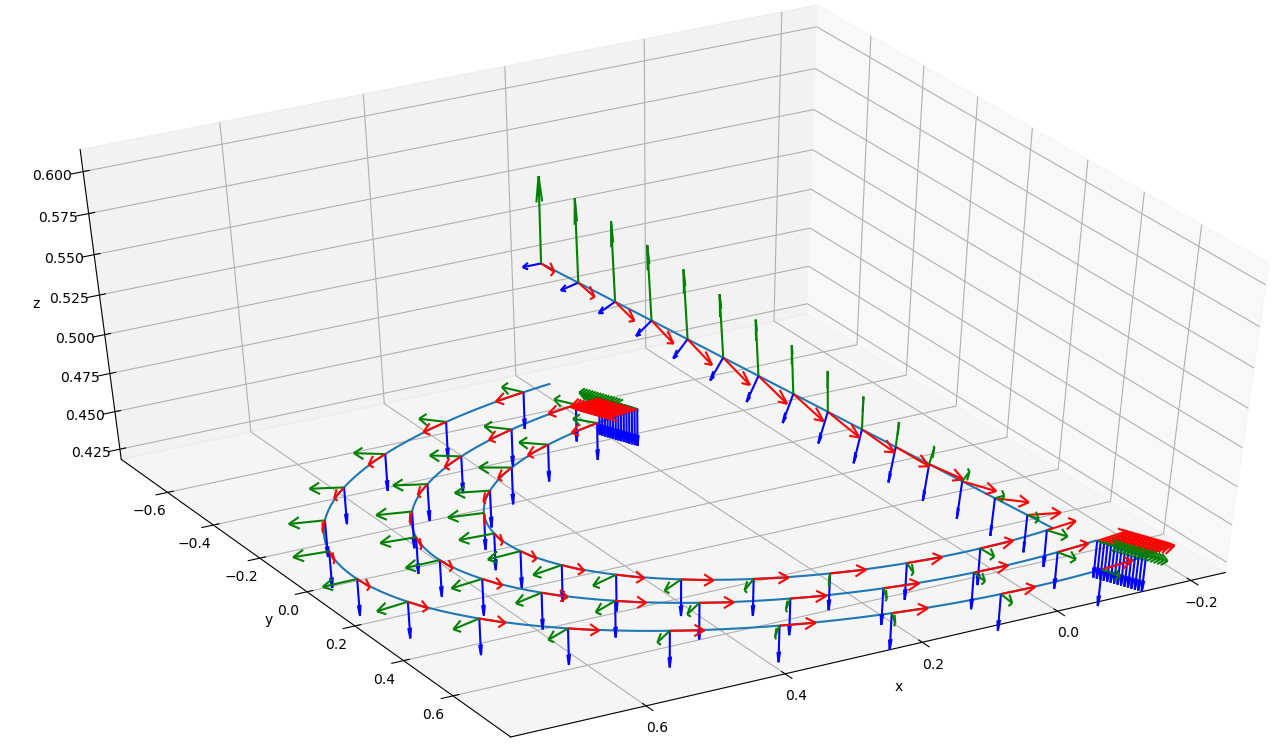
\includegraphics[keepaspectratio,width=0.9\textwidth]{scanning}
\caption{End-effector path and associated Frenet frames for the scanning phase.}
\end{figure}

\begin{figure}[h]
\centering
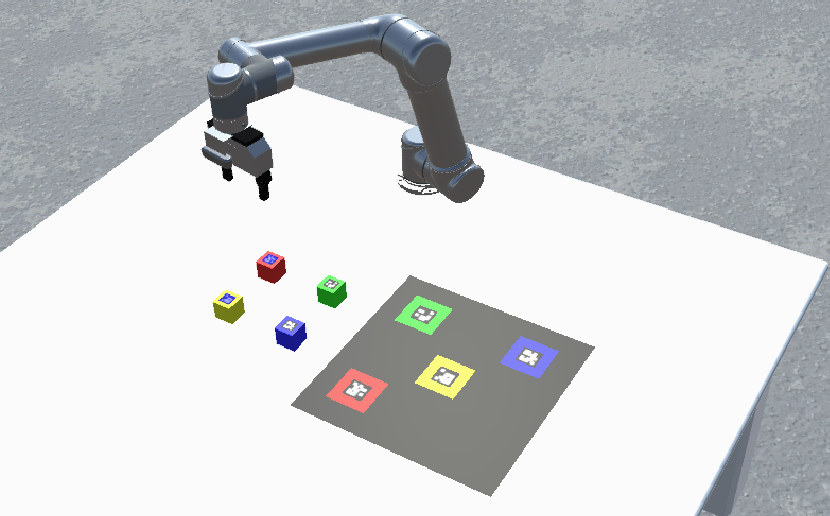
\includegraphics[keepaspectratio,width=0.6\textwidth]{scanning_sim}
\caption{Scanning task in Unity. The highlighted ARUCO markers are the ones currently detected by the end-effector camera.}
\end{figure}

\newpage

After the cubes and their destinations have been found, the pick-and-place phase is carried out as follows:

\begin{itemize}
\item Move linearly in Cartesian space towards the cube location.
\item Lower the end-effector onto the cube, close the gripper and then raise the end-effector back up.
\item Move linearly to the home position.
\item Move linearly to the destination, open the gripper and then raise the end-effector back up.
\item Move linearly to the home position.
\end{itemize}

\begin{figure}[h]
\centering
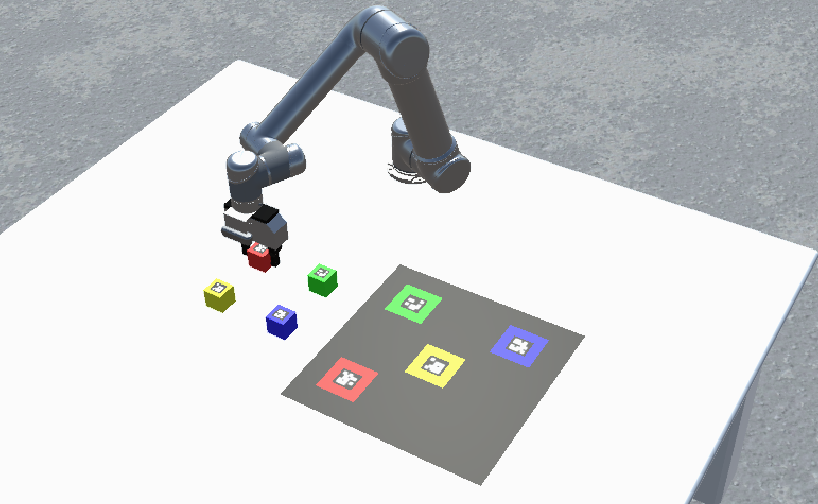
\includegraphics[keepaspectratio,width=0.4\textwidth]{pick}
\caption{Pick}
\end{figure}
\begin{figure}[h]
\centering
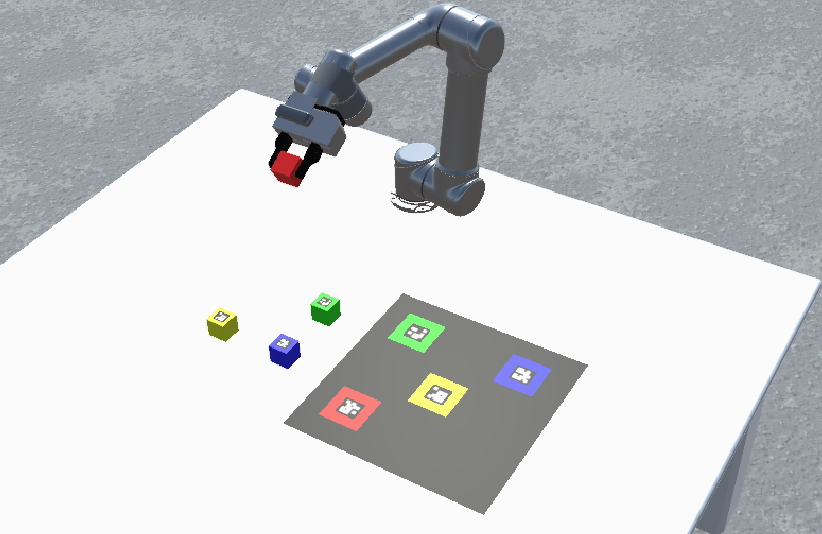
\includegraphics[keepaspectratio,width=0.4\textwidth]{home_w_cube}
\caption{Homing}
\end{figure}
\begin{figure}[h]
\centering
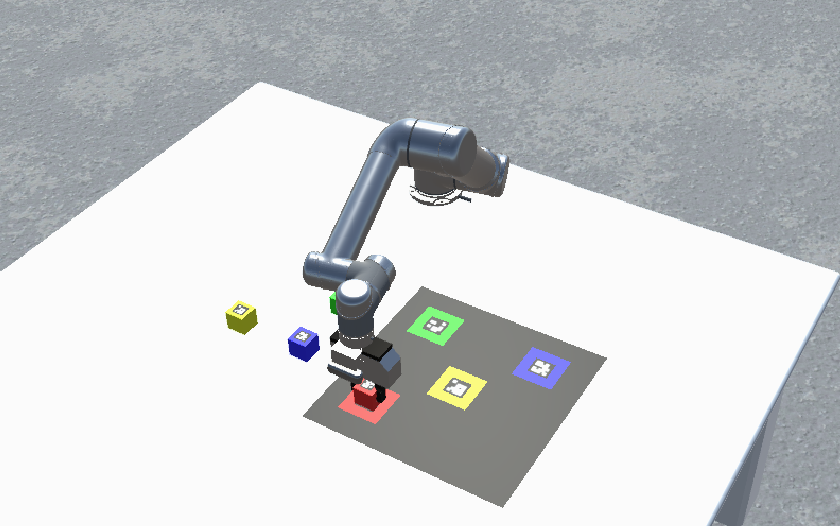
\includegraphics[keepaspectratio,width=0.4\textwidth]{place}
\caption{Place}
\end{figure}